\begin{figure}[h!]

  \setlength{\unitlength}{\textwidth}
  \fbox{
  \begin{picture}(1,0.35)(0,0.725)

    \put(-0.01,0.76){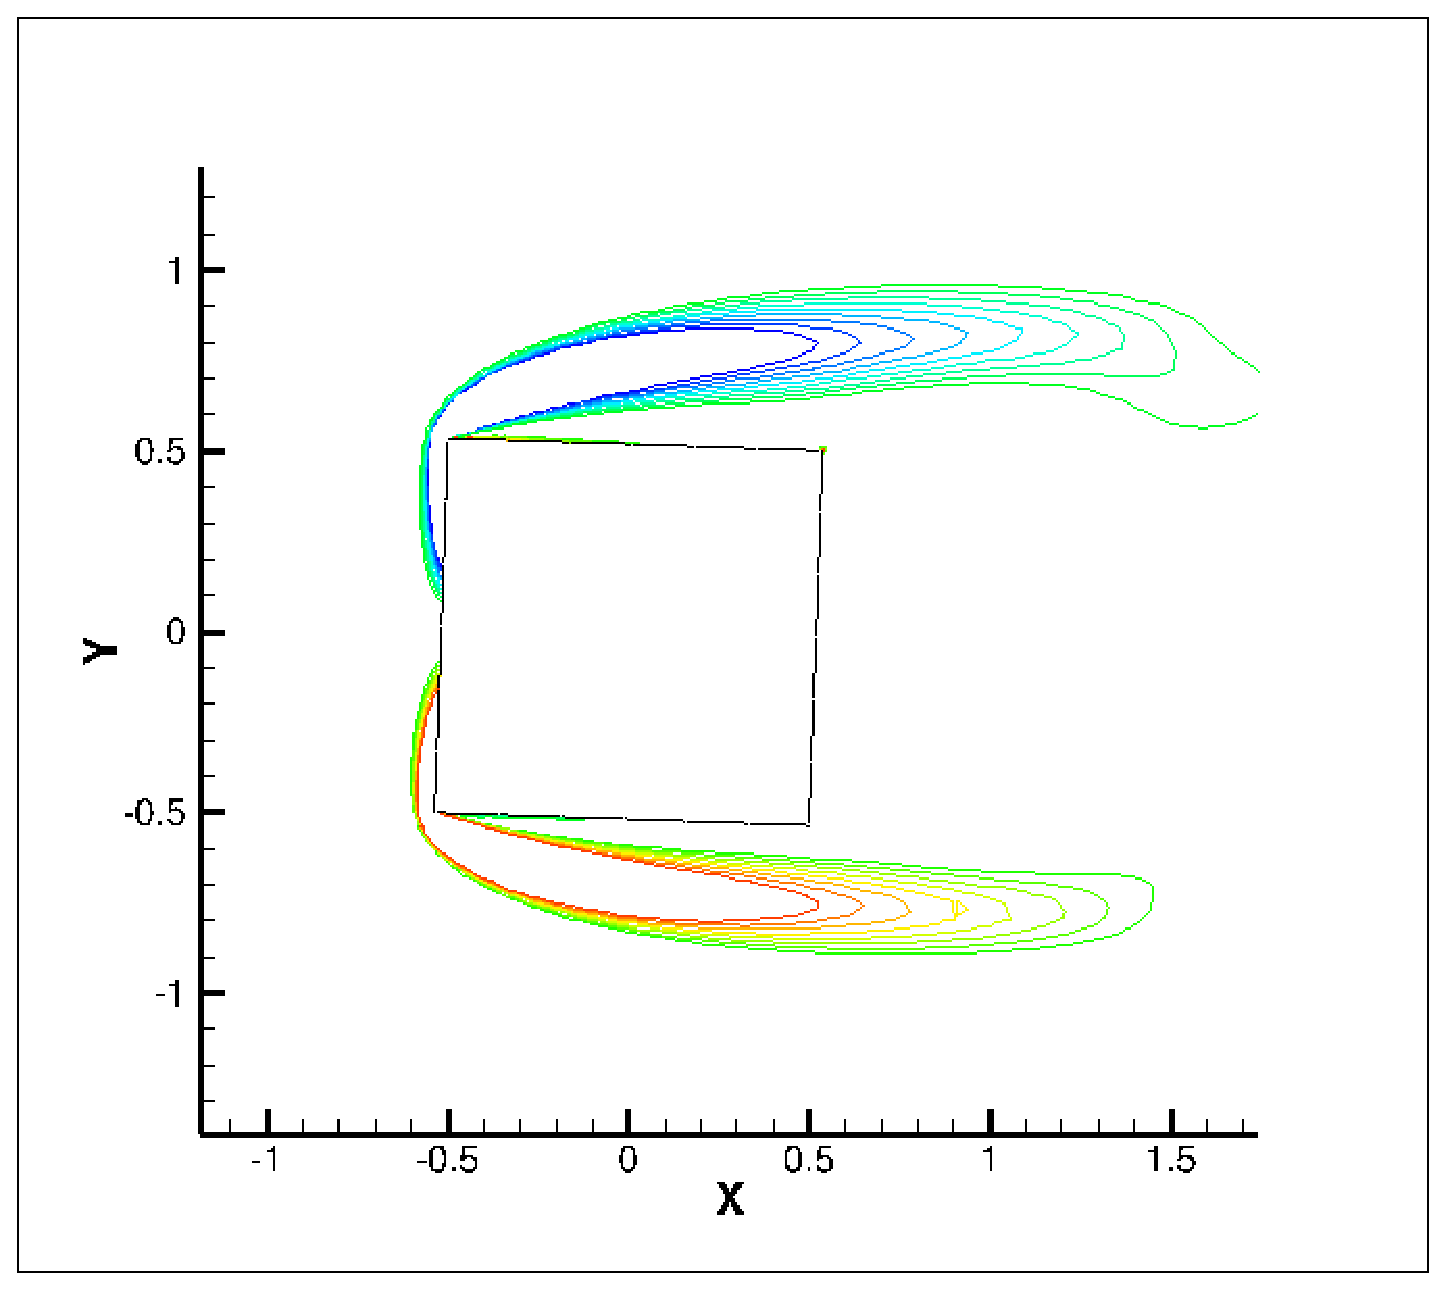
\includegraphics[width=0.33\unitlength]{./chapter-literature-revirw/fnp/square-2.eps}}
    \put(0.335,0.76){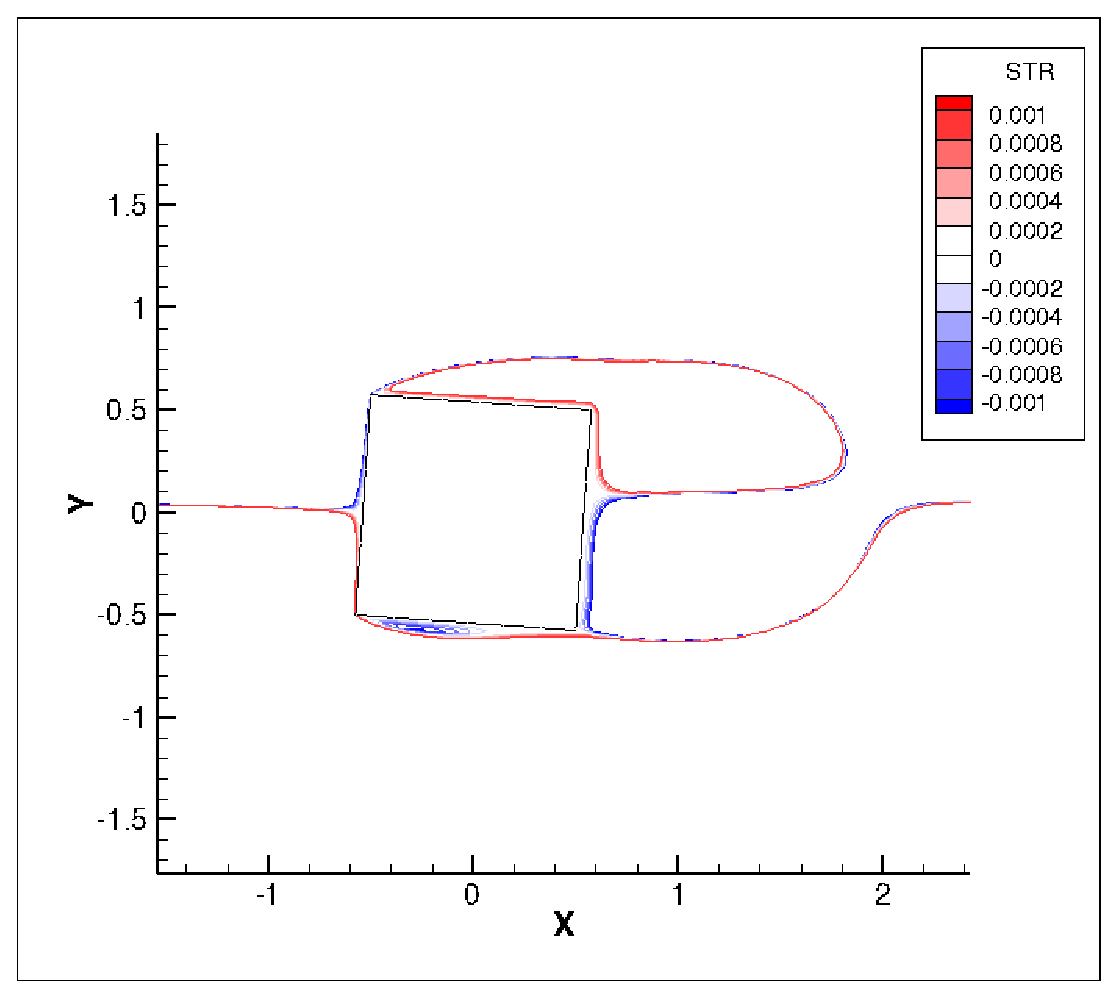
\includegraphics[width=0.33\unitlength]{./chapter-literature-revirw/fnp/square-4.eps}}
    \put(0.68,0.76){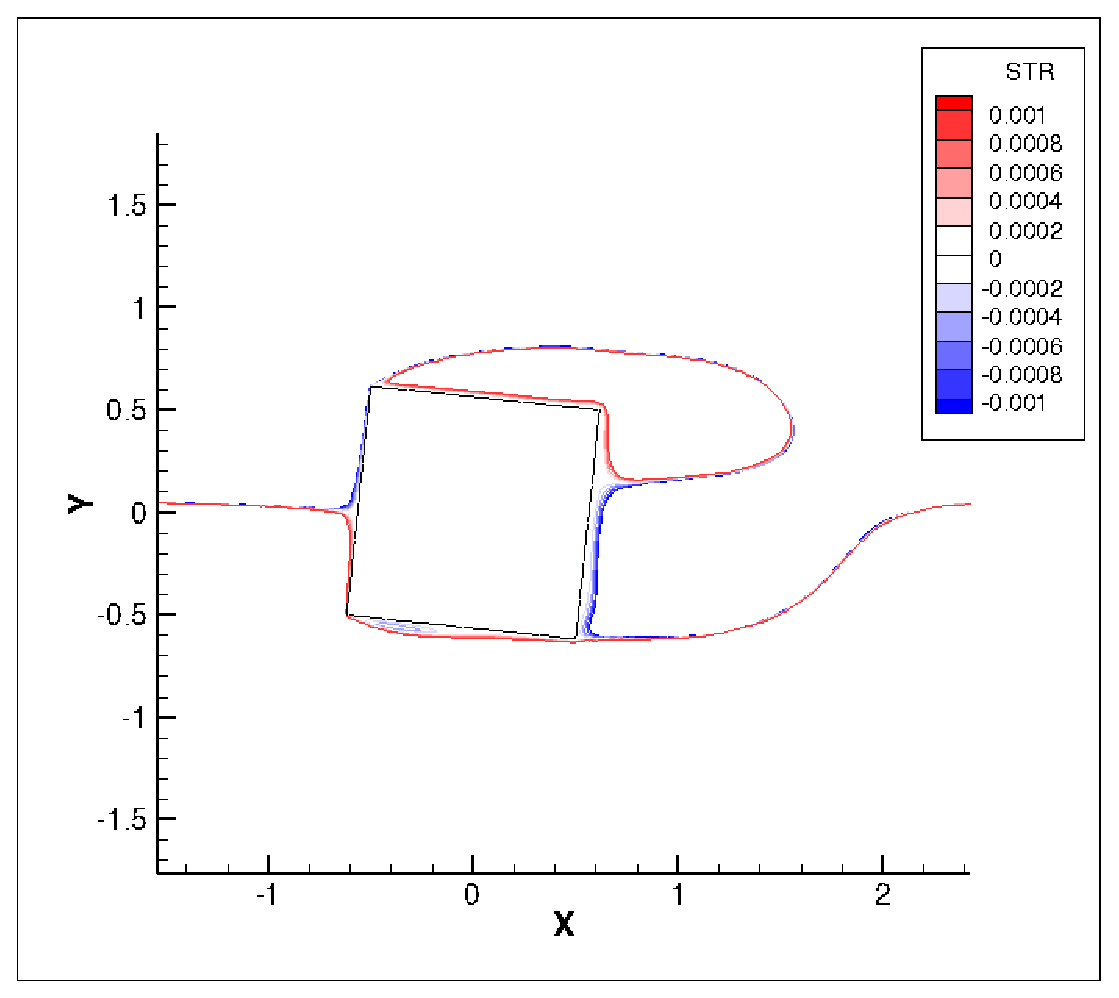
\includegraphics[width=0.33\unitlength]{.//chapter-literature-revirw/fnp/square-6.eps}}

   
    
    \put(0.0,0.735){(a)}    
    \put(0.34,0.735){(b)}
    \put(0.685,0.735){(c)}
  
  \end{picture}
}
  \caption{}
  \label{fig:shear_layers}
\end{figure}




